% Provenance (never printed): enseignement scientifique premiere (2019),
% "La Terre, un astre singulier" (the place of the Earth) and the old seconde
% SVT "La planete Terre, une planete habitable" (conditions for liquid water,
% the habitable zone); see sources/book2/PROVENANCE.md. Every temperature,
% phase boundary and habitable-zone limit is computed in
% figdata/grade-10/planet_temperatures.py.
\chapter{Un planeta habitable}\label{ch:g10:habitable-planet}

Tres planetas rocosos giran alrededor del Sol, uno junto a otro. En la
superficie de Venus, el aire es tan denso que presiona noventa y dos veces
más que en la Tierra, y tan caliente ---más de \qty{460}{\degreeCelsius}---
que el plomo se fundiría. En Marte, el aire tenue presiona menos de la
centésima parte que el nuestro, y la temperatura media está muy por debajo
del punto de congelación. Entre ambos, la Tierra tiene océanos, lluvia y
vida. Los tres planetas se formaron a partir del mismo disco de gas y polvo
que rodeaba al joven Sol, y casi de la misma roca. ¿Por qué destinos tan
distintos? Este capítulo estudia qué fija la temperatura de un planeta, qué
le permite conservar una atmósfera, en qué condiciones el agua puede ser
líquida y dónde, alrededor del Sol y de otras estrellas, se dan esas
condiciones.
% ledger: nasa:venus-atm, nasa:mars-atm, planet:Venus.Tmean

\begin{omfigure}
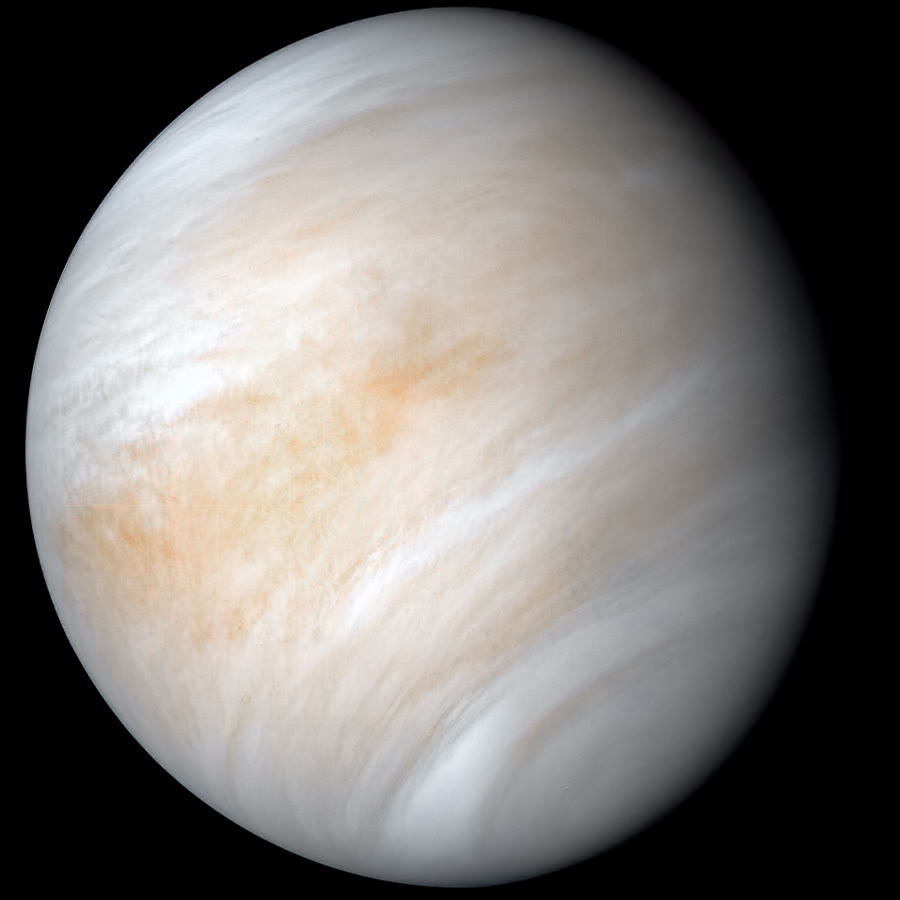
\includegraphics[width=0.38\linewidth]{images/book2/g10-nasa-venus-mariner10.jpg}

{\small Venus vista por la sonda Mariner~10 en 1974, con colores cercanos a
los que vería el ojo: un planeta envuelto por completo en nubes. Imagen:
NASA/JPL-Caltech (dominio público).}
\end{omfigure}

\begin{recall}
El Sol es una estrella; a su alrededor, los cuatro planetas rocosos
---Mercurio, Venus, la Tierra y Marte--- y después los cuatro planetas
gigantes recorren órbitas casi circulares (los libros de física y el
Libro 1). Todo cuerpo radia energía en forma de luz, tanto más cuanto más
alta es su temperatura, y sobre todo en forma de luz infrarroja a las
temperaturas de los planetas (los libros de física). Los gases de efecto
invernadero ---vapor de agua, dióxido de carbono, metano--- absorben parte
del infrarrojo que emite una superficie y la mantienen más caliente (los
libros de química). El agua existe como hielo, agua líquida y vapor de agua;
la presión es una fuerza por unidad de superficie, que se mide en pascales
(los libros de física).
\end{recall}

\section{La temperatura que fija la estrella}

El Sol envía su luz por igual en todas las direcciones. A una distancia $d$,
su potencia $L$ (su \emph{luminosidad}) se reparte sobre una esfera de área
$4\pi d^2$.

\begin{proposition}[La ley del inverso del cuadrado para la luz del Sol]\label{prop:g10:habitable-planet:inverse-square}
La potencia recibida por metro cuadrado de cara al Sol, la
\emph{irradiancia solar}, a una distancia $d$ del Sol es
\[
  S = \frac{L}{4\pi d^2}.
\]
A la distancia de la Tierra, \qty{1}{au}, $S_0 = \qty{1361}{W/m^2}$; a una
distancia $d$ medida en unidades astronómicas, $S = S_0/d^2$.
\end{proposition}

\begin{proof}
En el espacio vacío no se pierde luz, así que toda la potencia $L$ atraviesa
cada esfera centrada en el Sol; sobre una esfera de radio $d$ se reparte
entre $4\pi d^2$ metros cuadrados. Duplicar $d$ multiplica el área por cuatro
y divide $S$ entre cuatro.
\end{proof}
% ledger: earth:TSI, sun:L, const:au

\begin{omfigure}
\begin{tikzpicture}[font=\small, >={Stealth[length=2mm]}]
  \shade[ball color=yellow!70!orange] (0,0) circle (0.35);
  \node[below=4pt] at (0,-0.35) {Sol};
  \draw[omThm!70, thick] (0,0) -- (3,0.6) (0,0) -- (3,-0.6);
  \draw[omThm!70, thick, dashed] (3,0.6) -- (6,1.2) (3,-0.6) -- (6,-1.2);
  \draw[fill=omDef!25, draw=omDef!80!black] (3,-0.6) rectangle (3.18,0.6);
  \draw[fill=omDef!12, draw=omDef!80!black] (6,-1.2) rectangle (6.18,1.2);
  \draw[omDef!80!black] (6,0) -- (6.18,0) (6.09,-1.2) -- (6.09,1.2);
  \node[anchor=north] at (3.1,-0.7) {$d$};
  \node[anchor=north] at (6.1,-1.3) {$2d$};
  \node[anchor=south east, align=right, font=\footnotesize] at (2.9,0.75) {1 cuadrado:\\toda la luz};
  \node[anchor=west, align=left, font=\footnotesize] at (6.35,0.6) {4 cuadrados:\\un cuarto cada uno};
  \draw[->, black!60] (0.5,-1.95) -- (6.1,-1.95);
  \node[anchor=north, font=\footnotesize] at (3.3,-2.0) {distancia al Sol};
\end{tikzpicture}

{\small La luz que atraviesa un cuadrado a la distancia $d$ se reparte sobre
cuatro cuadrados del mismo tamaño a la distancia $2d$: la irradiancia
disminuye como el inverso del cuadrado de la distancia.}
\end{omfigure}

Un planeta absorbe la parte de esta luz que no refleja, y radia energía hacia
el espacio en forma de luz infrarroja. Si absorbe más de lo que radia, se
calienta; más caliente, radia más; y se estabiliza a la temperatura a la que
ambas cosas se equilibran.

\begin{definition}[Temperatura de equilibrio]\label{def:g10:habitable-planet:equilibrium-temperature}
La \emph{temperatura de equilibrio}\index{temperatura de equilibrio} de un
planeta es la temperatura a la que un cuerpo que radiara como un emisor
perfecto enviaría al espacio exactamente la potencia que el planeta absorbe
de su estrella. La fracción de la luz incidente que el planeta refleja en
conjunto es su \emph{albedo de Bond} $A$.
\end{definition}

\begin{proposition}[Cálculo de la temperatura de equilibrio]\label{prop:g10:habitable-planet:teq}
Para un planeta que reparte el calor que absorbe por toda su superficie,
\[
  T_{\mathrm{eq}} = \left(\frac{S\,(1-A)}{4\sigma}\right)^{1/4},
  \qquad \sigma = \qty{5.67e-8}{W.m^{-2}.K^{-4}}.
\]
A la distancia de la Tierra y sin ninguna reflexión, esto da
\qty{278.3}{K}; a una distancia $d$ en unidades astronómicas y con un albedo
$A$, $T_{\mathrm{eq}} = \qty{278.3}{K} \times (1-A)^{1/4}/\sqrt{d}$.
\end{proposition}

\begin{proof}[Demostración parcial]
El planeta intercepta la luz del Sol sobre un disco de área $\pi R^2$ y
absorbe la potencia $(1-A)\,S\,\pi R^2$. Radia por toda su superficie,
$4\pi R^2$. Un emisor perfecto a la temperatura $T$ radia $\sigma T^4$ por
metro cuadrado (una ley que se demuestra en los libros de física y que aquí
se admite). Igualar $4\pi R^2 \sigma T^4 = (1-A)\,S\,\pi R^2$ da la fórmula;
el radio se simplifica. Con $S = S_0/d^2$, la raíz cuarta de $1/d^2$ es
$1/\sqrt d$.
\end{proof}
% ledger: const:sigma, earth:TSI

\begin{example}[La Tierra]\label{ex:g10:habitable-planet:earth}
% ledger: earth:TSI, earth:albedo, earth:Tbb, earth:Tsurf
Con $S_0 = \qty{1361}{W/m^2}$ y $A = 0.294$,
$T_{\mathrm{eq}} = 278.3 \times 0.706^{1/4} \approx \qty{255}{K}$, es decir,
\qty{-18}{\degreeCelsius}. (La ficha de datos de la NASA da \qty{254}{K}.)
La temperatura media de la superficie terrestre es de \qty{288}{K},
\qty{15}{\degreeCelsius}: el efecto invernadero de la atmósfera la calienta
unos \qty{33}{K}. Sin él, los océanos se congelarían.
\end{example}

\begin{omfigure}
\begin{tikzpicture}
\begin{axis}[ybar, width=0.86\linewidth, height=5.8cm, ymin=0, ymax=950,
  bar width=10pt, enlarge x limits=0.15, symbolic x coords={Mercury,Venus,Earth,Moon,Mars},
  xticklabels={Mercurio,Venus,Tierra,Luna,Marte},
  xtick=data, ylabel={temperatura (K)}, ymajorgrids, grid style={gray!22},
  legend style={at={(0.97,0.95)}, anchor=north east, font=\footnotesize, draw=black!30},
  nodes near coords, nodes near coords style={font=\scriptsize, rotate=90, anchor=west, /pgf/number format/fixed, /pgf/number format/precision=0},
  tick label style={font=\small}, label style={font=\small}]
\addplot[fill=omDef!45, draw=omDef!80!black] table[x=name, y=Teq_K] {figdata/out/grade-10-planet_temperatures-planets.dat};
\addlegendentry{temperatura de equilibrio}
\addplot[fill=omThm!55, draw=omThm!80!black] table[x=name, y=Tmean_K] {figdata/out/grade-10-planet_temperatures-planets.dat};
\addlegendentry{temperatura media medida en la superficie}
\end{axis}
\end{tikzpicture}

{\small \omterm{def:g10:habitable-planet:equilibrium-temperature}{Temperaturas de equilibrio} calculadas a partir de la distancia y del
albedo de Bond de cada cuerpo, junto a las temperaturas medias medidas en su
superficie. Datos: fichas planetarias de la NASA.}
\end{omfigure}

\begin{remark}[Cómo leer el gráfico]\label{rem:g10:habitable-planet:reading}
% ledger: nasa:bond-albedos, planet:Mercury.Tmean, planet:Venus.Tmean, planet:Moon.Tmean, planet:Mars.Tmean, planet:Moon.day, nasa:moon-temps
En Mercurio y en Marte, que casi no tienen atmósfera o la tienen muy tenue,
la media medida se acerca a la \omterm{def:g10:habitable-planet:equilibrium-temperature}{temperatura de equilibrio}. La media de la Luna
queda por debajo: su día y su noche duran unas dos semanas cada uno, y su
superficie oscila entre unos \qty{95}{K} y \qty{390}{K}, algo que la fórmula
sencilla, pensada para un planeta que reparte su calor por igual, no
recoge. Venus es el caso llamativo: con un albedo de Bond de 0.77 ---sus
nubes reflejan la mayor parte de la luz del Sol---, su \omterm{def:g10:habitable-planet:equilibrium-temperature}{temperatura de
equilibrio} es más baja que la de la Tierra, y sin embargo su superficie está
más de \qty{500}{K} por encima: es el efecto invernadero de su densa
atmósfera de dióxido de carbono.
\end{remark}

\section{Conservar una atmósfera}

Un gas está formado por moléculas en movimiento constante, más rápido cuanto
más caliente está el gas. Una molécula de lo alto de una atmósfera que sube
más deprisa que la velocidad de escape del planeta ---la velocidad necesaria
para librarse de su gravedad para siempre (los libros de física)--- se
pierde en el espacio. A lo largo de miles de millones de años, un planeta
pequeño, de gravedad débil, pierde su aire; uno grande lo conserva.

\begin{center}
\small
% ledger: planet:Mercury.vesc, planet:Venus.vesc, planet:Earth.vesc, planet:Moon.vesc, planet:Mars.vesc, planet:Mercury.psurf, planet:Venus.psurf, planet:Earth.psurf, planet:Moon.psurf, nasa:mars-atm
\begin{tabular}{lccc}
\hline
cuerpo & velocidad de escape (\unit{km/s}) & presión en superficie (bar) & atmósfera \\
\hline
Luna & 2.4 & 0 & ninguna \\
Mercurio & 4.3 & 0 & ninguna \\
Marte & 5.0 & 0.006 & tenue, de dióxido de carbono \\
Venus & 10.4 & 92 & densa, de dióxido de carbono \\
Tierra & 11.2 & 1 & nitrógeno y oxígeno \\
\hline
\end{tabular}
\end{center}

\begin{remark}[El tamaño no lo explica todo]\label{rem:g10:habitable-planet:size}
La Luna y Mercurio, pequeños y (en el caso de Mercurio) cerca del ardiente
Sol, han perdido casi todos sus gases. Marte, con la mitad de la velocidad de
escape de la Tierra, conservó una atmósfera tenue. Venus y la Tierra tienen
casi el mismo tamaño y la misma velocidad de escape, pero atmósferas muy
distintas: sus historias ---el destino de su agua y de su dióxido de
carbono--- se separaron, como mostrará el \cref{ch:g12:early-earth} para la
Tierra.
\end{remark}

\section{El agua líquida}

\begin{omfigure}
\begin{tikzpicture}
\begin{axis}[omrecord, width=0.88\linewidth, height=7.2cm, xmin=150, xmax=800,
  ymode=log, ymin=1e-6, ymax=2000, xlabel={temperatura (K)}, ylabel={presión (bar)},
  xtick={200,300,...,800}, ytick={1e-6,1e-4,1e-2,1,100},
  log basis y=10]
\addplot[omDef!85!black, line width=1.1pt] table[x=T_K, y=p_bar] {figdata/out/grade-10-planet_temperatures-vap.dat};
\addplot[omDef!85!black, line width=1.1pt] table[x=T_K, y=p_bar] {figdata/out/grade-10-planet_temperatures-subl.dat};
\addplot[omDef!85!black, line width=1.1pt] table[x=T_K, y=p_bar] {figdata/out/grade-10-planet_temperatures-melt.dat};
\addplot[only marks, mark=*, mark size=2pt, black] coordinates {(273.16,0.00611657) (647.096,220.64)};
\addplot[only marks, mark=square*, mark size=2.4pt, omThm!85!black] table[x=T_K, y=p_bar] {figdata/out/grade-10-planet_temperatures-points.dat};
\node[font=\small] at (axis cs:205,30) {hielo};
\node[font=\small] at (axis cs:420,30) {líquido};
\node[font=\small] at (axis cs:600,1e-3) {vapor de agua};
\node[font=\footnotesize, anchor=north west] at (axis cs:276,0.0055) {punto triple};
\node[font=\footnotesize, anchor=south east] at (axis cs:640,300) {punto crítico};
\node[font=\footnotesize, anchor=south, omThm!85!black] at (axis cs:737,110) {Venus};
\node[font=\footnotesize, anchor=west, omThm!85!black] at (axis cs:296,1.0) {Tierra};
\node[font=\footnotesize, anchor=north, omThm!85!black] at (axis cs:210,0.0045) {Marte};
\end{axis}
\end{tikzpicture}

{\small Diagrama de fases del agua, con las condiciones medias en la
superficie de Venus, la Tierra y Marte (cuadrados). El eje de presiones es
logarítmico: cada marca vale cien veces la anterior. Curvas calculadas con
las ecuaciones de la International Association for the Properties of Water
and Steam; valores planetarios de la NASA.}
\end{omfigure}

\begin{proposition}[Cuándo puede ser líquida el agua]\label{prop:g10:habitable-planet:liquid}
% ledger: iapws:triple-critical, iapws:vapour-pressure, iapws:melt-subl
El agua líquida solo existe a presiones superiores a la del \emph{punto
triple}, \qty{611.657}{Pa} (\qty{0.006}{bar}), en el que coexisten hielo,
líquido y vapor a \qty{273.16}{K}, y a temperaturas inferiores a la del
\emph{punto crítico}, \qty{647.096}{K} (\qty{220.64}{bar}), más allá del
cual ya no se pueden distinguir el líquido y el vapor. A una presión dada
por encima del punto triple, el agua es líquida entre su punto de fusión,
cercano a \qty{273}{K}, y su punto de ebullición, que baja a medida que baja
la presión.
\end{proposition}

\begin{example}[Tres planetas en un mismo diagrama]\label{ex:g10:habitable-planet:three}
% ledger: nasa:venus-atm, nasa:mars-atm, earth:psurf, earth:Tsurf (boiling point at 636 Pa computed)
La superficie de la Tierra, a \qty{288}{K} y \qty{1}{bar}, queda dentro del
campo del líquido: el agua puede estar allí líquida, helada o en vapor según
el tiempo que haga. Venus, a \qty{737}{K}, queda muy por encima de la
temperatura crítica: allí no es posible el agua líquida en absoluto. Marte,
a \qty{6.36}{mbar}, queda justo por encima del punto triple: el agua hierve
allí a unos \qty{0.5}{\degreeCelsius}, así que el agua líquida solo podría
sobrevivir en una ventana de medio grado, y la temperatura media,
\qty{210}{K}, está en el campo del hielo.
\end{example}

\begin{omfigure}
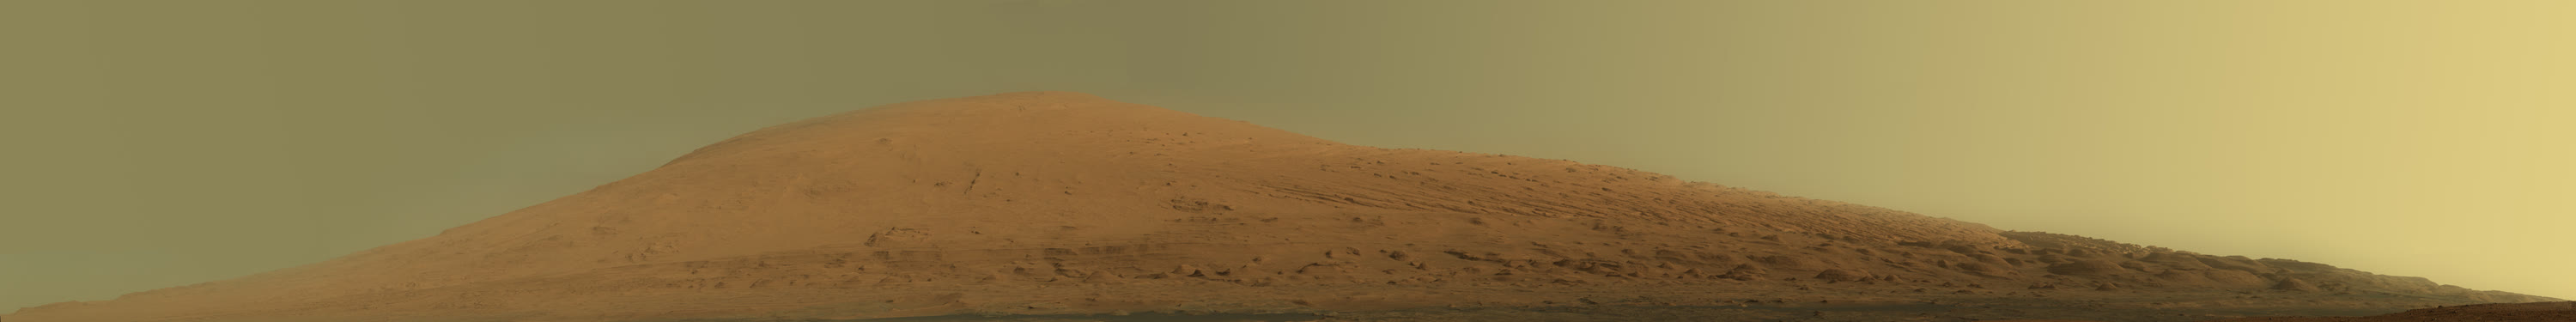
\includegraphics[width=0.96\linewidth]{images/book2/g10-nasa-mars-mount-sharp.jpg}

{\small El monte Sharp, dentro del cráter Gale de Marte, fotografiado por el
róver Curiosity en 2012, con los colores que registró su cámara. Sus capas
inferiores se depositaron en el agua hace miles de millones de años. Imagen:
NASA/JPL-Caltech/MSSS (dominio público).}
\end{omfigure}

\section{La zona habitable}

\begin{definition}[Zona habitable]\label{def:g10:habitable-planet:habitable-zone}
La \emph{zona habitable}\index{zona habitable} de una estrella es el
intervalo de distancias a la estrella en el que un planeta rocoso con agua
suficiente y una atmósfera como la de la Tierra podría conservar agua
líquida en su superficie. Su borde interior está donde el planeta perdería
su agua por el calor; su borde exterior, donde ni siquiera un fuerte efecto
invernadero podría ya impedir que se congelara.
\end{definition}

\begin{proposition}[La zona habitable del Sol]\label{prop:g10:habitable-planet:hz-sun}
% ledger: kopparapu:hz-sun, planet:Mercury.dist, planet:Venus.dist, planet:Mars.dist
Los modelos detallados de atmósferas planetarias sitúan la \omterm{def:g10:habitable-planet:habitable-zone}{zona habitable}
del Sol entre \qty{0.99}{au} y \qty{1.70}{au}. La Tierra (\qty{1}{au}) está
justo por dentro de su borde interior; Marte (\qty{1.52}{au}) está dentro de
ella; Venus (\qty{0.72}{au}) queda muy por dentro del borde interior.
\end{proposition}

\begin{proposition}[Zonas habitables de otras estrellas]\label{prop:g10:habitable-planet:hz-scaling}
Alrededor de una estrella de luminosidad $L$, un planeta recibe la misma
irradiancia que a una distancia $d_\odot$ del Sol cuando se encuentra a
\[
  d = d_\odot \sqrt{L/L_\odot}.
\]
Los bordes de la \omterm{def:g10:habitable-planet:habitable-zone}{zona habitable} se desplazan en la misma proporción, en
primera aproximación (el color de la luz de la estrella también influye un
poco).
\end{proposition}

\begin{proof}
Igual irradiancia significa $L/(4\pi d^2) = L_\odot/(4\pi d_\odot^2)$, luego
$d^2 = d_\odot^2\,L/L_\odot$.
\end{proof}

\begin{omfigure}
\begin{tikzpicture}[font=\small]
  % top: the Sun, 0-2 au over 12 cm (6 cm per au)
  \fill[omProp!30] (0.99*6,0) rectangle (1.70*6,0.5);
  \draw[black!70] (0,0.25) -- (12.3,0.25);
  \foreach \x in {0,0.5,...,2} \draw (\x*6,0.15) -- (\x*6,0.35) node[pos=0, below=1pt, font=\footnotesize] {\x};
  \shade[ball color=yellow!70!orange] (0,0.25) circle (0.22);
  \foreach \n/\d in {Mercurio/0.387, Venus/0.723, Tierra/1.0, Marte/1.524} {
    \fill[omThm!85!black] (\d*6,0.25) circle (2.2pt);
    \node[anchor=south, font=\footnotesize] at (\d*6,0.55) {\n};
  }
  \node[anchor=west, font=\footnotesize] at (12.4,0.25) {au};
  \node[anchor=north, font=\footnotesize] at (8.07,-0.25) {zona habitable, 0.99--1.70 au};
  \node[anchor=east, font=\footnotesize] at (-0.3,0.25) {Sol};
  % bottom: Proxima Centauri, 0-0.1 au over 12 cm (120 cm per au)
  \begin{scope}[yshift=-2.2cm]
  \fill[omProp!30] (0.0385*120,0) rectangle (0.0661*120,0.5);
  \draw[black!70] (0,0.25) -- (12.3,0.25);
  \foreach \x/\l in {0/0, 0.025/0.025, 0.05/0.05, 0.075/0.075, 0.1/0.1} \draw (\x*120,0.15) -- (\x*120,0.35) node[pos=0, below=1pt, font=\footnotesize] {\l};
  \shade[ball color=red!70!orange] (0,0.25) circle (0.14);
  \fill[omThm!85!black] (0.0485*120,0.25) circle (2.2pt);
  \node[anchor=south, font=\footnotesize] at (0.0485*120,0.55) {Próxima b};
  \node[anchor=west, font=\footnotesize] at (12.4,0.25) {au};
  \node[anchor=north, font=\footnotesize] at (6.28,-0.25) {zona habitable, 0.038--0.066 au};
  \node[anchor=east, align=right, font=\footnotesize] at (-0.3,0.25) {Próxima\\Centauri};
  \end{scope}
\end{tikzpicture}

{\small Arriba: la \omterm{def:g10:habitable-planet:habitable-zone}{zona habitable} del Sol y los cuatro planetas rocosos.
Abajo: la \omterm{def:g10:habitable-planet:habitable-zone}{zona habitable} de la débil estrella roja Próxima Centauri,
calculada escalando la del Sol con la raíz cuadrada de la luminosidad de la
estrella, y su planeta Próxima~b. Fíjate en el cambio de escala: toda la
banda de abajo mide \qty{0.1}{au}.}
\end{omfigure}

\section{Planetas de otras estrellas}

\begin{definition}[Exoplaneta]\label{def:g10:habitable-planet:exoplanet}
Un \emph{exoplaneta}\index{exoplaneta} es un planeta que gira alrededor de
una estrella distinta del Sol.
\end{definition}

Los \omterm{def:g10:habitable-planet:exoplanet}{exoplanetas} son demasiado débiles y están demasiado cerca de sus
estrellas para verse directamente, salvo algunos gigantes. La mayoría se
descubren de forma indirecta: o bien el planeta pasa por delante de su
estrella una vez en cada órbita y la atenúa muy ligeramente, o bien su
atracción hace que la estrella oscile acercándose y alejándose de nosotros,
lo que desplaza alternativamente el color de su luz. El segundo método solo
da una masa \emph{mínima} para el planeta, porque no se conoce la
inclinación de la órbita. Estos métodos se estudian en el volumen del
tercer año universitario.

\begin{dated}{2026}
% ledger: nea:count-2026
El 15 de octubre de 2026, el NASA Exoplanet Archive recogía 6\,451
\omterm{def:g10:habitable-planet:exoplanet}{exoplanetas} confirmados.
\end{dated}

\begin{example}[Próxima b]\label{ex:g10:habitable-planet:proxima}
% ledger: nea:proxima-b (flux and habitable zone computed in figdata/grade-10/planet_temperatures.py)
La estrella más cercana al Sol, Próxima Centauri, a \qty{1.30}{\parsec}, es
una pequeña estrella roja cuya luminosidad es solo unas $0.0015$ veces la del
Sol. En 2016 se descubrió un planeta que la rodea cada 11.2 días, a
\qty{0.0485}{au}, con al menos 1.06 veces la masa de la Tierra. A esa
distancia recibe unas 0.64 veces la irradiancia que recibe la Tierra, y se
encuentra dentro de la \omterm{def:g10:habitable-planet:habitable-zone}{zona habitable} de su estrella. No se sabe si tiene
atmósfera, ni agua.
\end{example}

\begin{remark}[Habitable no quiere decir habitado]\label{rem:g10:habitable-planet:inhabited}
La \omterm{def:g10:habitable-planet:habitable-zone}{zona habitable} es una afirmación solo sobre la distancia y la luz. Un
planeta situado en ella puede no tener agua, ni atmósfera, o tener una
inadecuada: Marte está dentro de la zona del Sol y hoy no tiene agua líquida
en su superficie. La Tierra es habitable porque se cumplen a la vez varias
condiciones: la distancia adecuada, una masa suficiente para conservar una
atmósfera, agua abundante y un efecto invernadero ni demasiado débil ni
demasiado fuerte.
\end{remark}

\section{Ejercicios}

\begin{exercise}[$\star$]\label{exo:g10:habitable-planet:1}
Define la \omterm{def:g10:habitable-planet:equilibrium-temperature}{temperatura de equilibrio} de un planeta. ¿Por qué la temperatura
media de la superficie terrestre es más alta que su \omterm{def:g10:habitable-planet:equilibrium-temperature}{temperatura de
equilibrio}?
\end{exercise}

\begin{exercise}[$\star$]\label{exo:g10:habitable-planet:2}
Con el diagrama de barras de las \omterm{def:g10:habitable-planet:equilibrium-temperature}{temperaturas de equilibrio} y medidas, nombra
el cuerpo cuya superficie calienta más su atmósfera, y estima en cuántos
kelvin.
\end{exercise}

\begin{exercise}[$\star$]\label{exo:g10:habitable-planet:3}
Marte gira a \qty{1.52}{au} del Sol. Con la ley del inverso del cuadrado y
$S_0 = \qty{1361}{W/m^2}$, calcula la irradiancia solar en Marte.
\end{exercise}

\begin{exercise}[$\star$]\label{exo:g10:habitable-planet:4}
Con el diagrama de fases del agua, indica el estado del agua a \qty{1}{bar}
y \qty{330}{K}; a \qty{0.001}{bar} y \qty{250}{K}; a \qty{100}{bar} y
\qty{700}{K}.
\end{exercise}

\begin{exercise}[$\star$]\label{exo:g10:habitable-planet:5}
¿Qué es un \omterm{def:g10:habitable-planet:exoplanet}{exoplaneta}? Describe en una frase cada uno de los dos métodos
principales con los que se detectan \omterm{def:g10:habitable-planet:exoplanet}{exoplanetas}.
\end{exercise}

\begin{exercise}[$\star\star$]\label{exo:g10:habitable-planet:6}
Calcula la \omterm{def:g10:habitable-planet:equilibrium-temperature}{temperatura de equilibrio} de la Tierra con
$S_0 = \qty{1361}{W/m^2}$ y $A = 0.294$, y después con $A = 0$. Convierte
ambas a grados Celsius.
\end{exercise}

\begin{exercise}[$\star\star$]\label{exo:g10:habitable-planet:7}
Una estrella es cuatro veces más luminosa que el Sol. ¿Entre qué distancias
se encuentra su \omterm{def:g10:habitable-planet:habitable-zone}{zona habitable}? ¿Estaría dentro la Tierra, colocada a
\qty{1}{au} de ella?
\end{exercise}

\begin{exercise}[$\star\star$]\label{exo:g10:habitable-planet:8}
Venus gira a \qty{0.723}{au}. Calcula la irradiancia que recibe y después su
\omterm{def:g10:habitable-planet:equilibrium-temperature}{temperatura de equilibrio} con su albedo de Bond de 0.77. Compárala con su
temperatura superficial de \qty{737}{K} y explica la diferencia.
\end{exercise}

\begin{exercise}[$\star\star$]\label{exo:g10:habitable-planet:9}
En Marte, la presión media en la superficie es de \qty{6.36}{mbar}, justo
por encima del punto triple del agua, y el agua hierve allí a unos
\qty{0.5}{\degreeCelsius}. Explica por qué el agua líquida no puede durar
hoy en la superficie de Marte, ni siquiera una tarde de verano en la que el
suelo alcance \qty{10}{\degreeCelsius}.
\end{exercise}

\begin{exercise}[$\star\star$]\label{exo:g10:habitable-planet:10}
La velocidad de escape es de \qty{2.4}{km/s} en la Luna y de
\qty{11.2}{km/s} en la Tierra. Calcula su cociente. Explica por qué la
Tierra ha conservado una atmósfera y la Luna no.
\end{exercise}

\begin{exercise}[$\star\star$]\label{exo:g10:habitable-planet:11}
Supón que la Tierra se cubriera de hielo y que su albedo de Bond subiera a
0.50. Calcula su nueva \omterm{def:g10:habitable-planet:equilibrium-temperature}{temperatura de equilibrio}. Explica por qué un estado
así, una vez alcanzado, tendería a mantenerse.
\end{exercise}

\begin{exercise}[$\star\star\star$]\label{exo:g10:habitable-planet:12}
Demuestra que $T_{\mathrm{eq}} = \qty{278.3}{K} \times (1-A)^{1/4}/\sqrt{d}$,
con $d$ en unidades astronómicas, se deduce de la fórmula del capítulo. ¿Por
qué factor cambia la \omterm{def:g10:habitable-planet:equilibrium-temperature}{temperatura de equilibrio} cuando la distancia se
multiplica por cuatro?
\end{exercise}

\begin{exercise}[$\star\star\star$]\label{exo:g10:habitable-planet:13}
¿A qué distancia del Sol tendría un planeta de albedo 0.294 una \omterm{def:g10:habitable-planet:equilibrium-temperature}{temperatura
de equilibrio} de \qty{273}{K}? Compárala con el borde interior de la \omterm{def:g10:habitable-planet:habitable-zone}{zona
habitable} y explica por qué las dos son distintas.
\end{exercise}

\begin{exercise}[$\star\star\star$]\label{exo:g10:habitable-planet:14}
En un planeta cuya presión en la superficie es de \qty{1000}{Pa}, el agua
hierve a unos \qty{7}{\degreeCelsius}. ¿Entre qué temperaturas puede ser
líquida el agua allí? ¿Qué le pasaría a un lago de ese planeta un día a
\qty{15}{\degreeCelsius}?
\end{exercise}

\begin{exercise}[$\star\star\star$]\label{exo:g10:habitable-planet:15}
Un planeta gira a \qty{1.2}{au} de una estrella la mitad de luminosa que el
Sol. Calcula los bordes de la \omterm{def:g10:habitable-planet:habitable-zone}{zona habitable} de la estrella y di si el
planeta está dentro. ¿Hasta qué punto puede uno estar seguro de la
respuesta?
\end{exercise}

\section{Problema: ¿podría Próxima b albergar un océano?}

\begin{problem}[{Problema de fin de semana --- de la luz de una débil
estrella roja a la temperatura de su planeta más cercano}]
\label{pb:g10:habitable-planet:1}
% ledger: nea:proxima-b, kopparapu:hz-sun, earth:TSI, earth:albedo, planet:Earth.vesc, nasa:bond-albedos (all results computed in figdata/grade-10/planet_temperatures.py or from the rounded data below)
Un estudiante lee la ficha de datos del planeta Próxima~b. Su estrella tiene
una luminosidad $L = 0.00151\,L_\odot$; el planeta gira a
$d = \qty{0.0485}{au}$ en 11.18 días y tiene al menos 1.055 veces la masa de
la Tierra. Usa $S_0 = \qty{1361}{W/m^2}$,
$\sigma = \qty{5.67e-8}{W.m^{-2}.K^{-4}}$, la \omterm{def:g10:habitable-planet:habitable-zone}{zona habitable} del Sol,
\qtyrange{0.99}{1.70}{au}, y la velocidad de escape de la Tierra,
\qty{11.2}{km/s}.

\medskip
\noindent\textbf{Parte I --- La luz de la estrella.}
\begin{enumerate}
  \item Calcula la irradiancia que recibe el planeta como fracción de la de
        la Tierra, $L/d^2$ (con $L$ en luminosidades solares y $d$ en au).
  \item Exprésala en \unit{W/m^2}.
  \item Compárala con la irradiancia en Venus (\qty{2601}{W/m^2}) y en
        Marte (\qty{586}{W/m^2}).
  \item ¿Cuántos años del planeta caben en un año terrestre?
\end{enumerate}

\medskip
\noindent\textbf{Parte II --- Temperaturas sin atmósfera.}
\begin{enumerate}[resume]
  \item Calcula la \omterm{def:g10:habitable-planet:equilibrium-temperature}{temperatura de equilibrio} de un planeta perfectamente
        oscuro ($A = 0$) con esa irradiancia.
  \item Calcúlala para un planeta tan brillante como Venus ($A = 0.77$).
  \item ¿Cuál de estas dos temperaturas está por encima del punto de
        congelación del agua? ¿Qué muestran los dos resultados sobre el
        papel de las nubes y del hielo?
\end{enumerate}

\medskip
\noindent\textbf{Parte III --- La zona habitable.}
\begin{enumerate}[resume]
  \item Calcula $\sqrt{L/L_\odot}$.
  \item Calcula el borde interior de la \omterm{def:g10:habitable-planet:habitable-zone}{zona habitable} de la estrella.
  \item Calcula su borde exterior.
  \item ¿Está Próxima~b dentro de la \omterm{def:g10:habitable-planet:habitable-zone}{zona habitable}?
  \item ¿A qué distancia del Sol recibiría un planeta la misma irradiancia
        que Próxima~b? ¿En qué parte de la \omterm{def:g10:habitable-planet:habitable-zone}{zona habitable} del Sol estaría?
\end{enumerate}

\medskip
\noindent\textbf{Parte IV --- ¿Una atmósfera y agua?}
\begin{enumerate}[resume]
  \item Si el planeta tuviera la densidad media de la Tierra, su radio sería
        $1.055^{1/3}$ veces el terrestre. Calcula este factor.
  \item La velocidad de escape es proporcional a $\sqrt{M/R}$. Estima la
        velocidad de escape del planeta. ¿Podría conservar una atmósfera?
  \item ¿Por qué solo se conoce un valor mínimo de la masa?
  \item En el diagrama de fases, ¿cuál es la presión mínima en la superficie
        que permitiría la existencia de agua líquida?
  \item Calcula la \omterm{def:g10:habitable-planet:equilibrium-temperature}{temperatura de equilibrio} de Próxima~b con el albedo de
        la Tierra, 0.294.
  \item ¿En cuántos kelvin tendría que calentarla entonces su efecto
        invernadero para llevar su superficie a la temperatura media de la
        Tierra, \qty{288}{K}?
\end{enumerate}
\end{problem}
